\documentclass[12pt]{article}
\usepackage{lecture}
\usepackage{graphicx}
\usepackage{html}
\usepackage{url}
\usepackage{epstopdf}

\renewcommand{\myurl}[1]{\htmladdnormallink{#1}{#1}}

\newcommand{\copyrightYears}{2008}

\title{Analysis of mismatch distributions}

\begin{document}

\maketitle

\thispagestyle{first}

\section*{Introduction}

Remember when we were talking about Tajima's $D$?\footnote{Don't
  answer that. I don't think I want to know the answer.} I pointed out
that $\hat \theta_\pi$, the estimate of $4N_e\mu$ derived from
nucleotide sequence diversity is less sensitive to demographic changes
than $\hat \theta_k$, the estimate of $4N_e\mu$ derived from the
number of segregating sites in the sample. I went on to argue that in
a rapidly expanding population, mutation will not have ``built up''
the level of nucleotide diversity we'd expect based on the number of
segregating sites, so that $\hat D = \theta_\pi - \theta_k$ will be
negative. In a population that's suffered a recent bottleneck, on the
other hand, there will be more nucleotide diversity than we'd expect
on the basis of the number of segregating sites, so that $\hat D$ will
be positive.

Figures 1--3 may help you to visualize what's going on. We get to
revisit our old friend the
coalescent. Figure~\ref{fig:coalescent-constant} shows the genealogical
relationships among a set of alleles sampled from two different
populations that exchange genes every other generation, on average
that haven't changed size. The four different coalescent trees
correspond to four different loci. The red and green dots correspond
to the different populations from which the alleles were collected.

\begin{figure}
\begin{center}
\resizebox{!}{5cm}{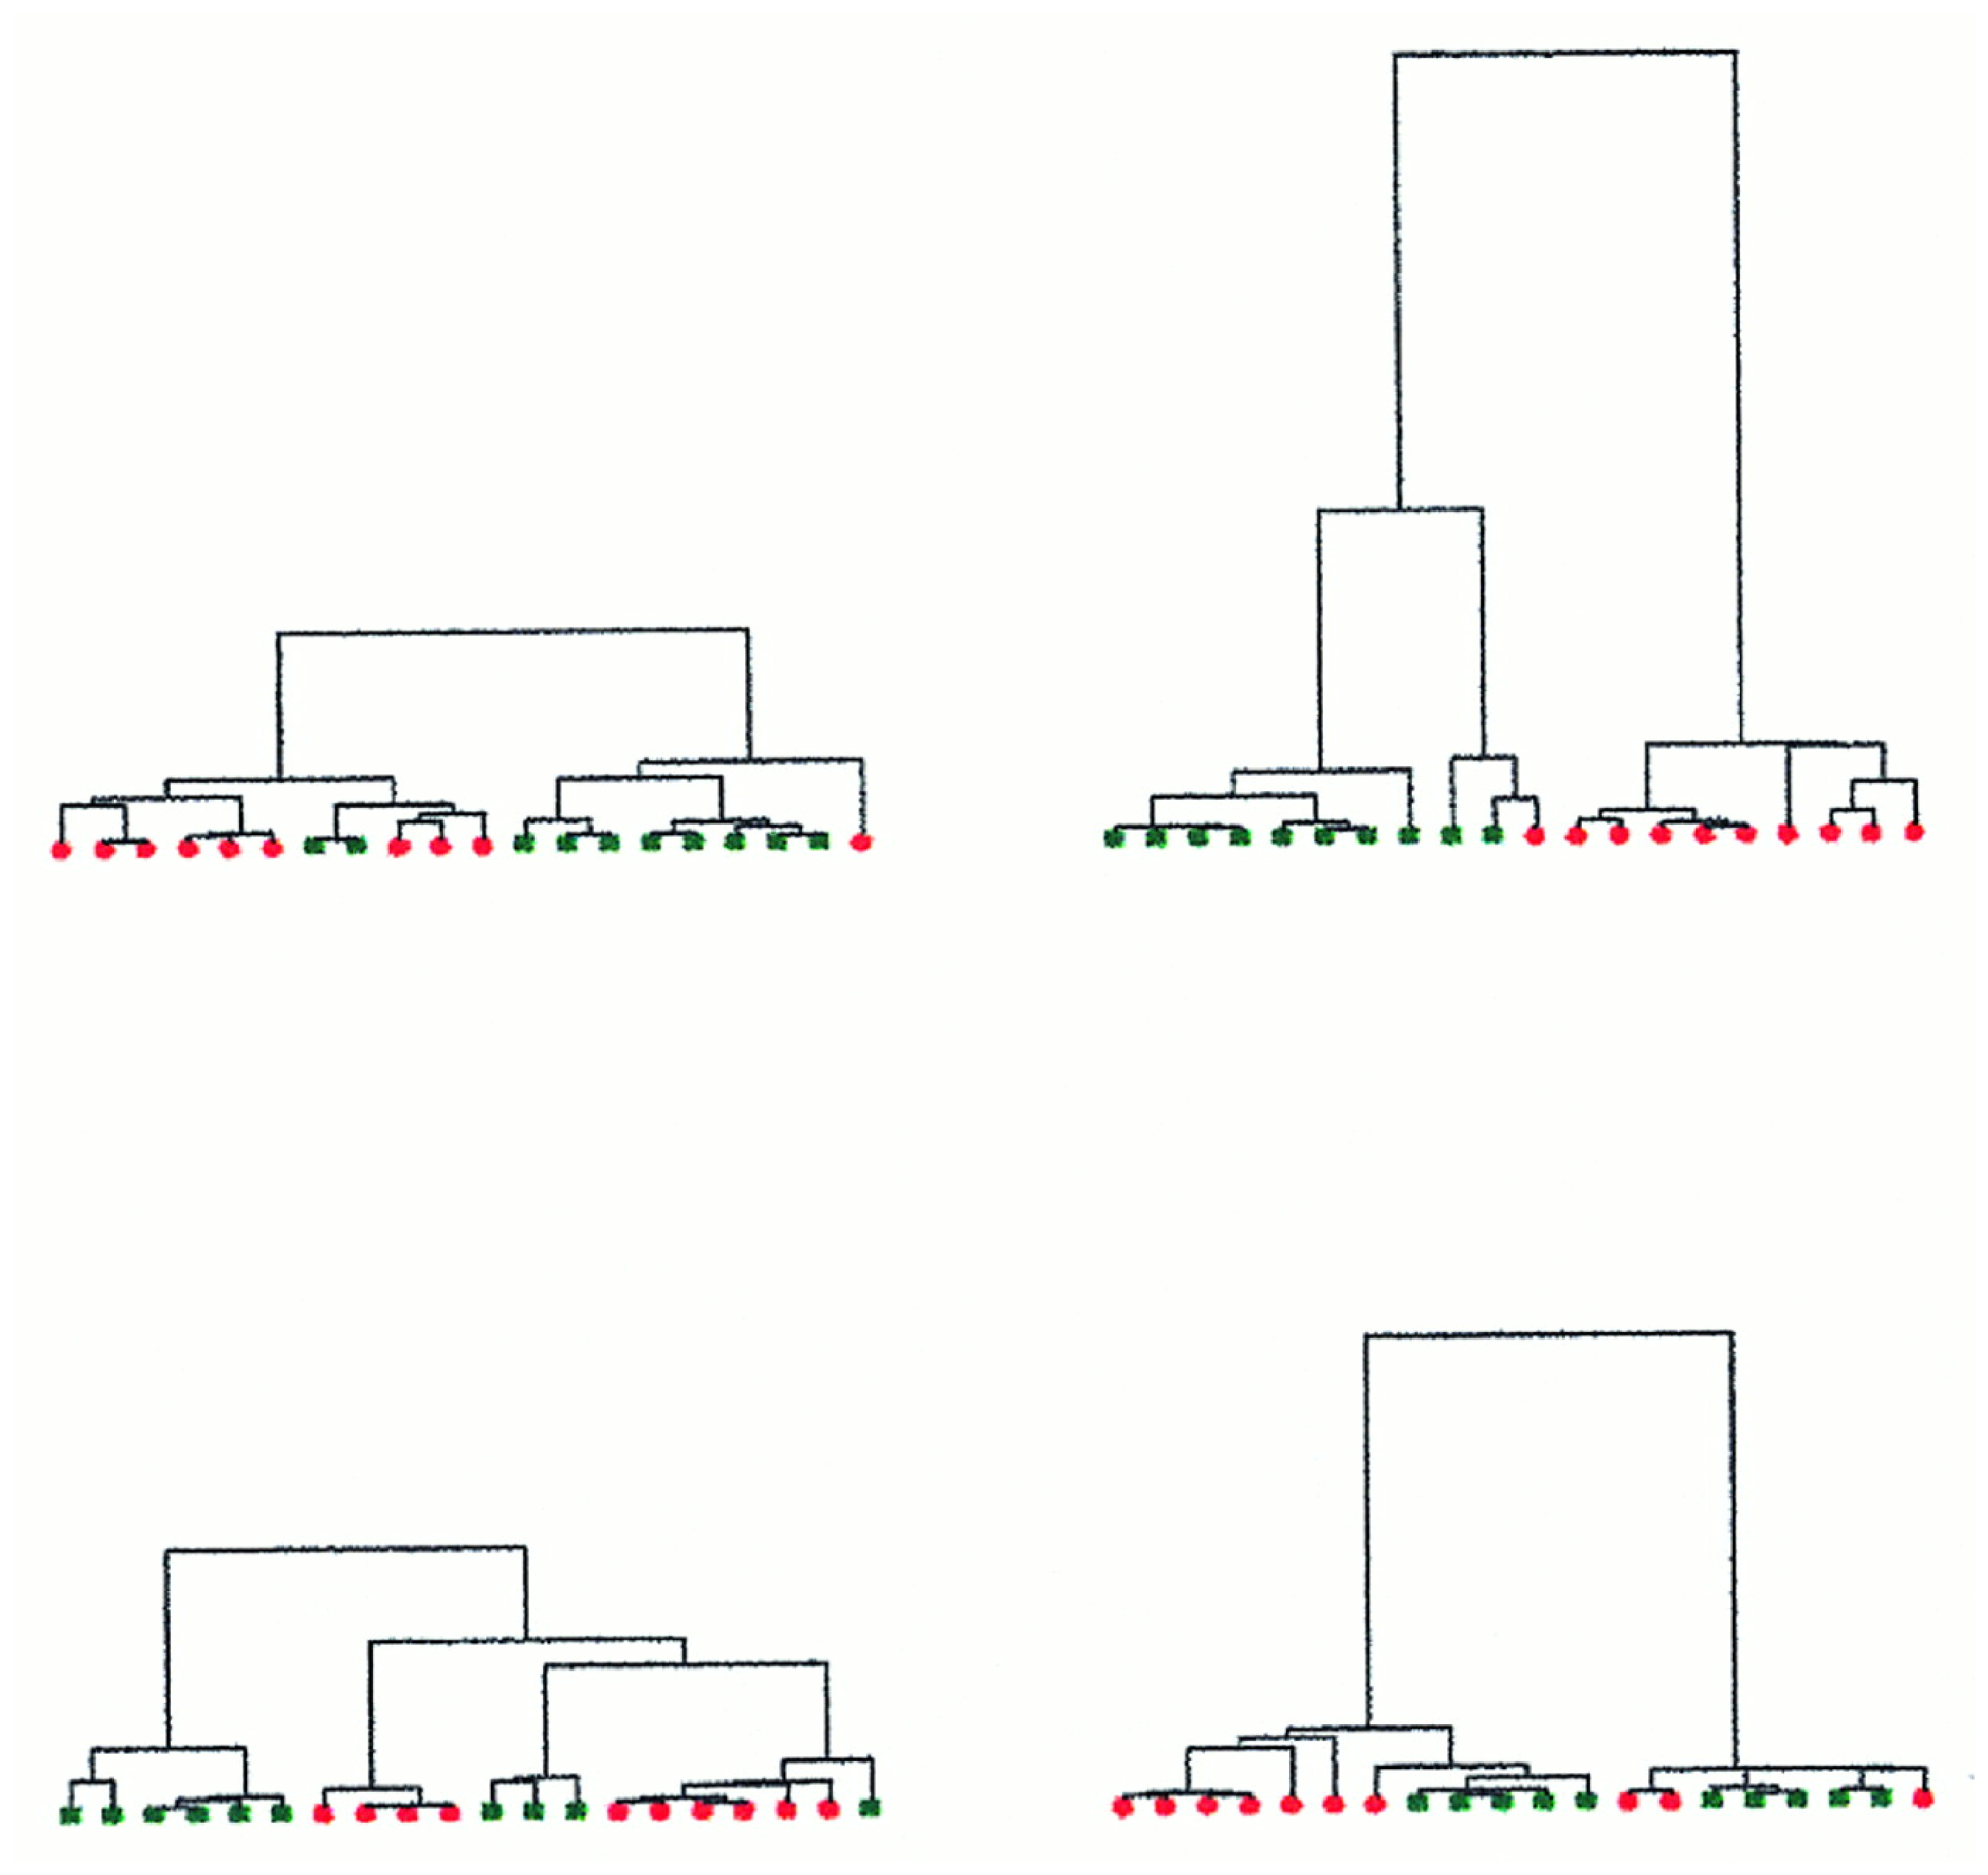
\includegraphics{coalescent-constant.eps}}
\end{center}
\caption{Four simulated coalescent trees for a sample of alleles from
  two populations of constant size that exchange genes every other
  generation on average (from~\cite{Harpending-etal-1998}).}\label{fig:coalescent-constant}
\end{figure}

Looking at Figure~\ref{fig:coalescent-constant} isn't particularly
revealing by itself, except that it shows how much variability there
is in coalescent history among loci, even when the demographic
parameters. What's more interesting is to compare those trees with
similar trees generated when the populations have undergone either a
recent expansion~(Figure~\ref{fig:coalescent-expansion}) or a recent
contraction~(Figure~\ref{fig:coalescent-contraction}). As you can see,
when populations have undergone a recent expansion, all of the
branches are relatively long. When they've undergone a recent
bottleneck, on the other hand, all of the branches are quite
short.

\begin{figure}
\begin{center}
\resizebox{!}{5cm}{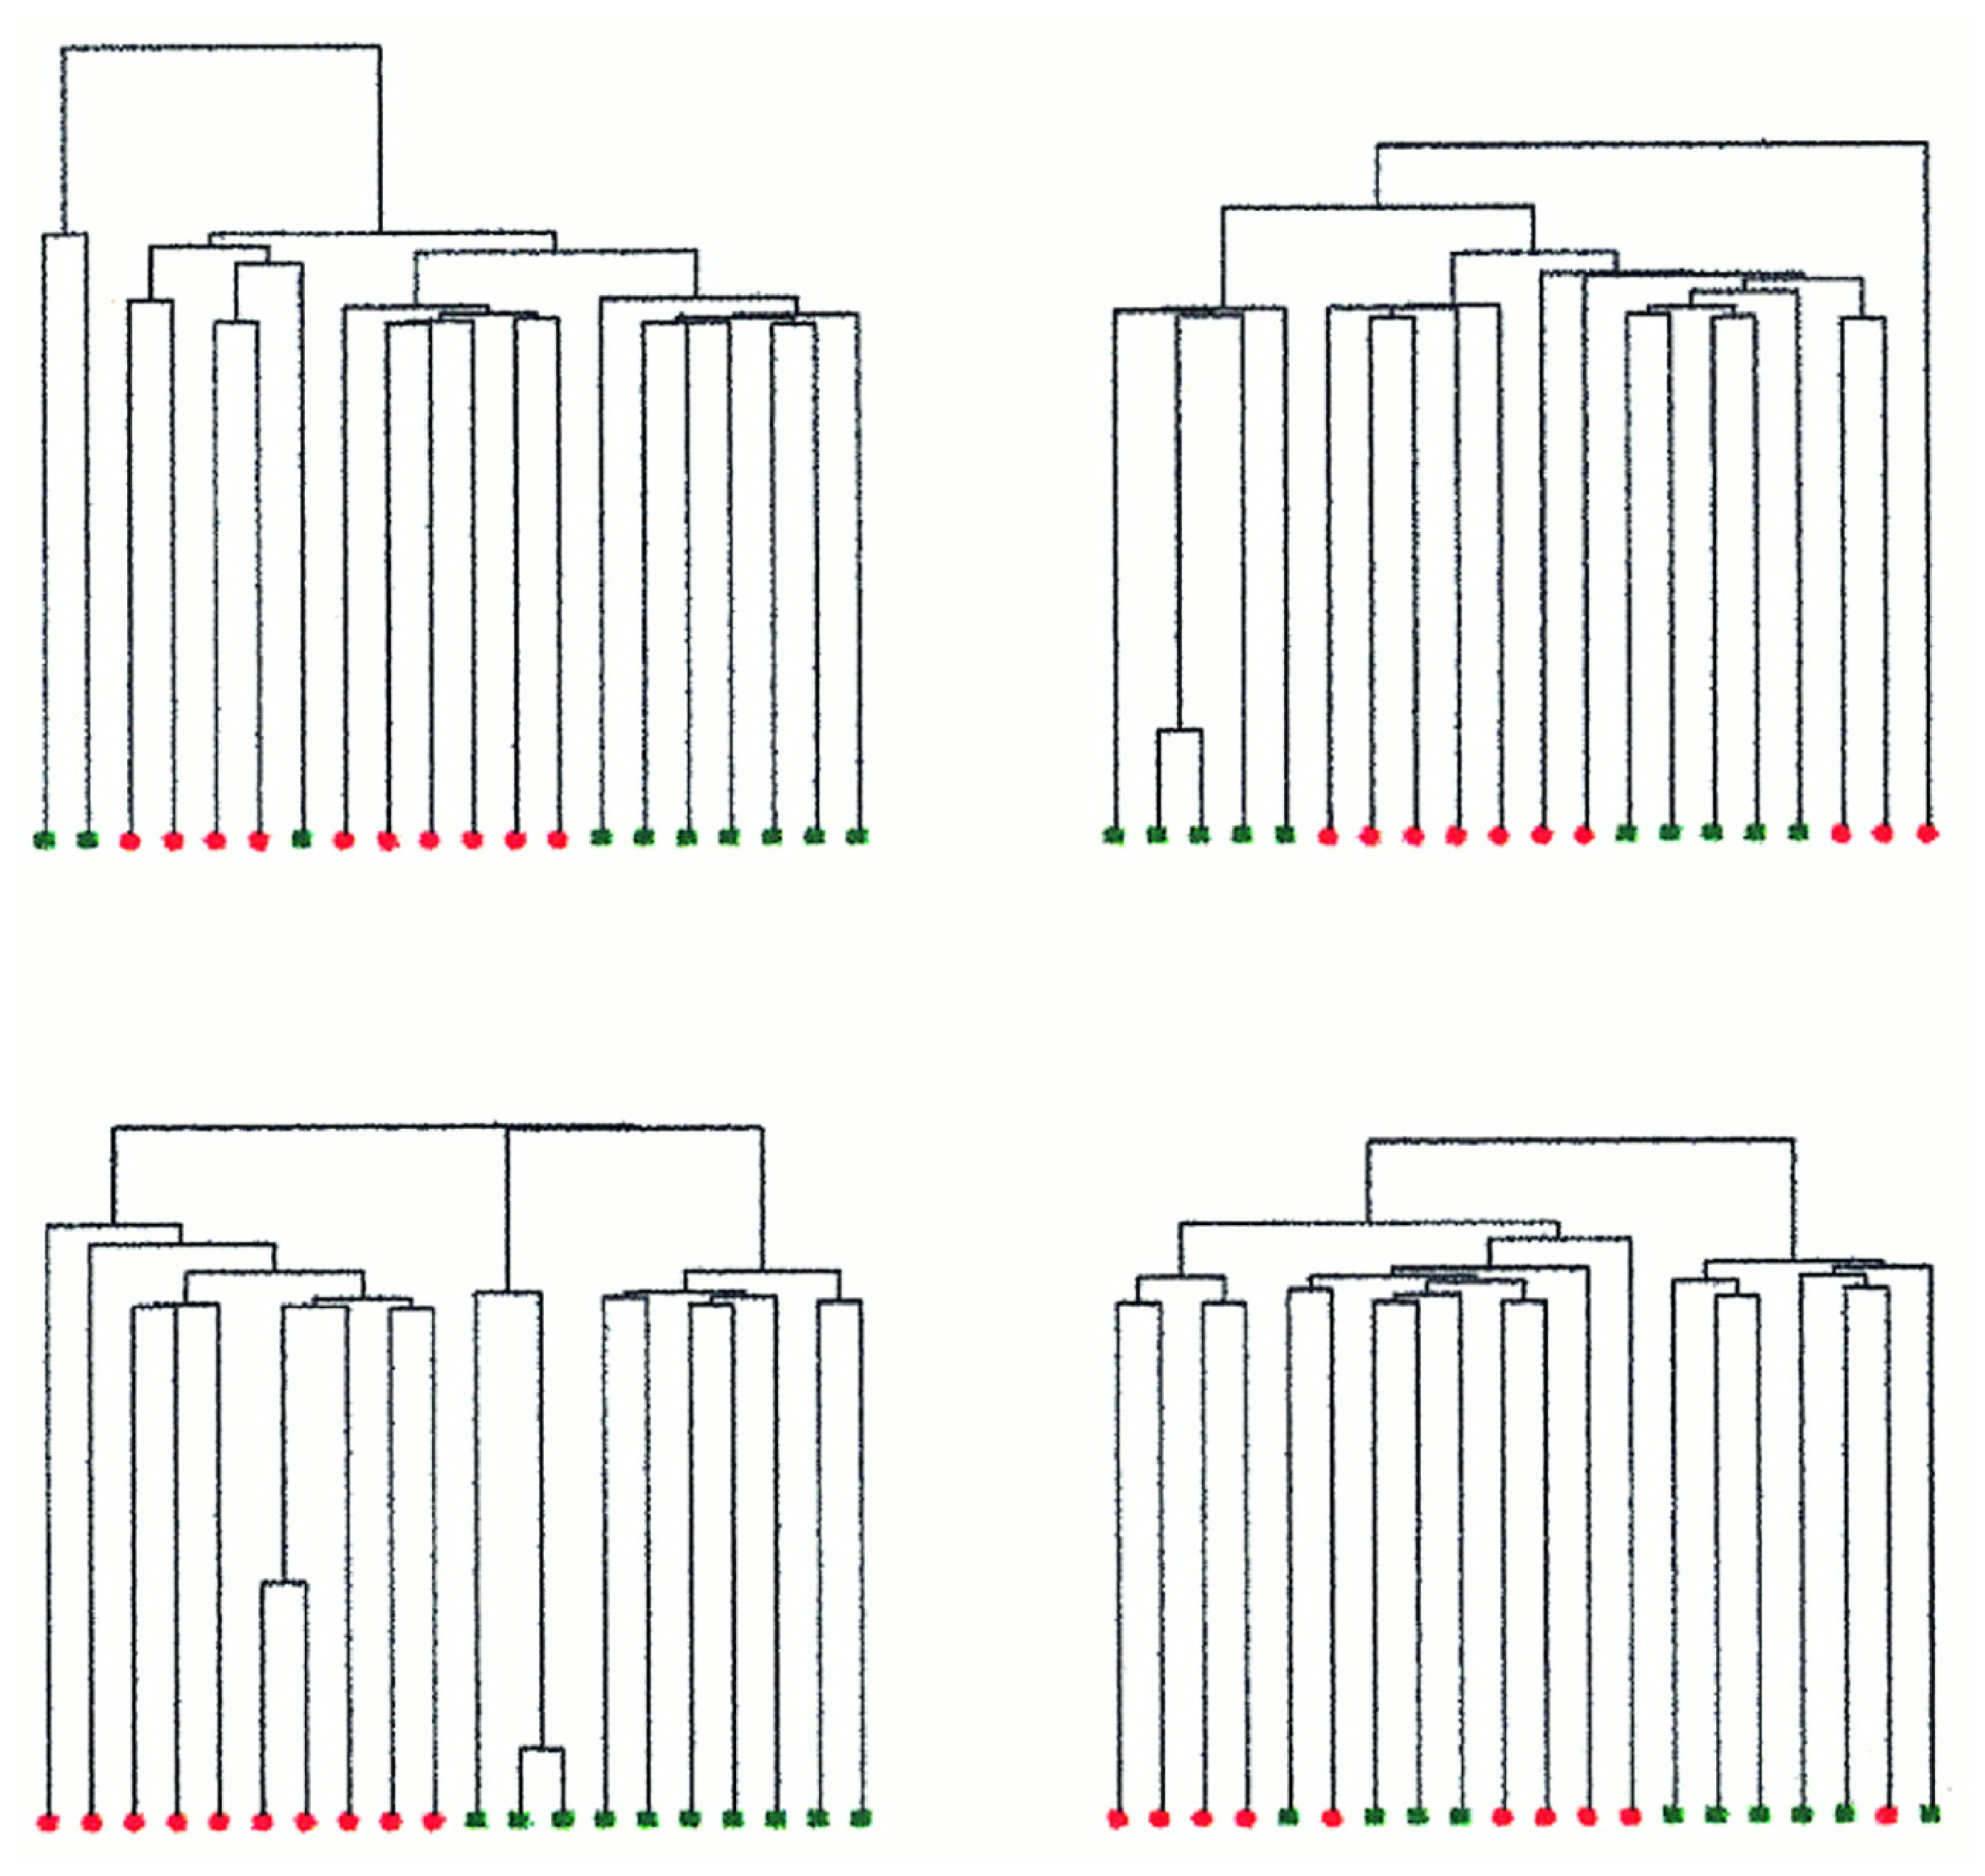
\includegraphics{coalescent-expansion.eps}}
\end{center}
\caption{Four simulated coalescent trees for a sample of alleles from
  two populations that have undergone a recent expansion and exchange
  genes every other generation on average
  (from~\cite{Harpending-etal-1998}).}\label{fig:coalescent-expansion} 
\end{figure}

\begin{figure}
\begin{center}
\resizebox{!}{5cm}{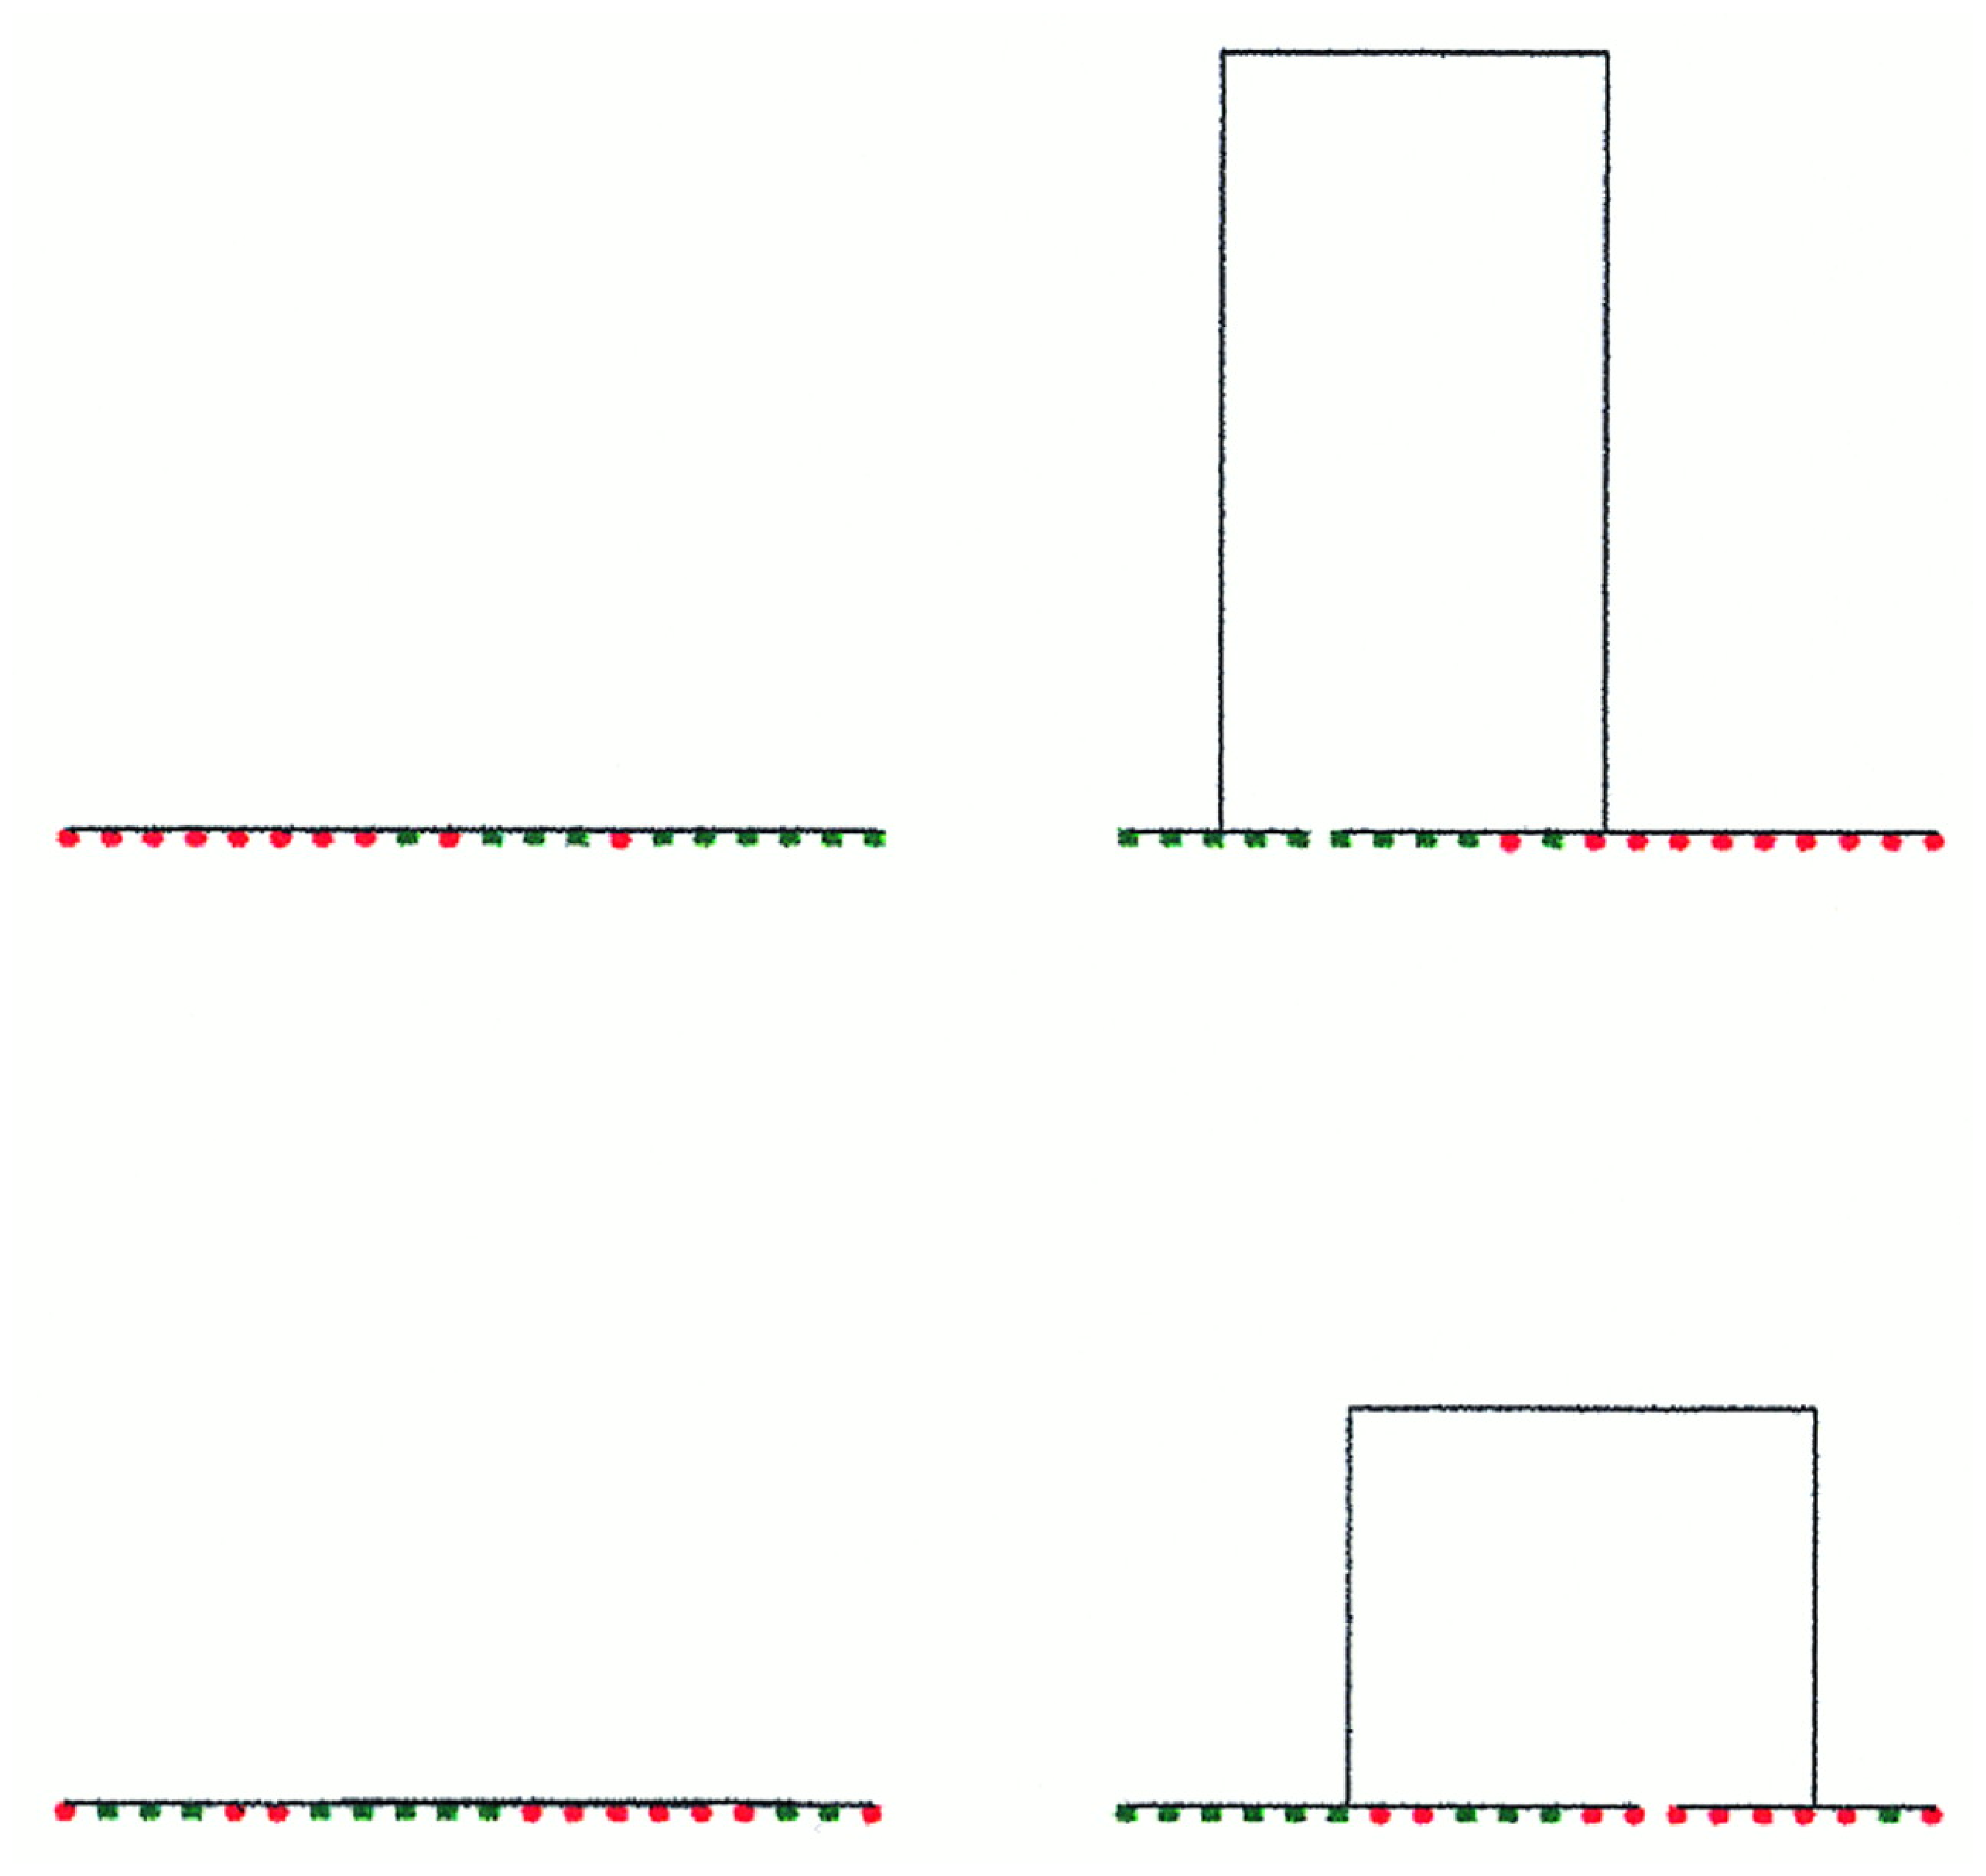
\includegraphics{coalescent-contraction.eps}}
\end{center}
\caption{Four simulated coalescent trees for a sample of alleles from
  two populations that have undergone a recent contraction and exchange
  genes every other generation on average
  (from~\cite{Harpending-etal-1998}).}\label{fig:coalescent-contraction} 
\end{figure}

\section*{Mismatch distributions}

Since the amount of sequence difference between alleles depends on the
length of time since they diverged, these observations suggest that we
might be able to learn more about the recent demographic history of
populations by looking not just at a summary statistic like
$\theta_\pi$ or $\theta_k$, but at the whole distribution of sequence
differences. In fact, as Figure~\ref{fig:mismatch-constant} and
Figure~\ref{fig:mismatch-expansion} show, the differences are quite
dramatic.

\begin{figure}
\begin{center}
\resizebox{!}{5cm}{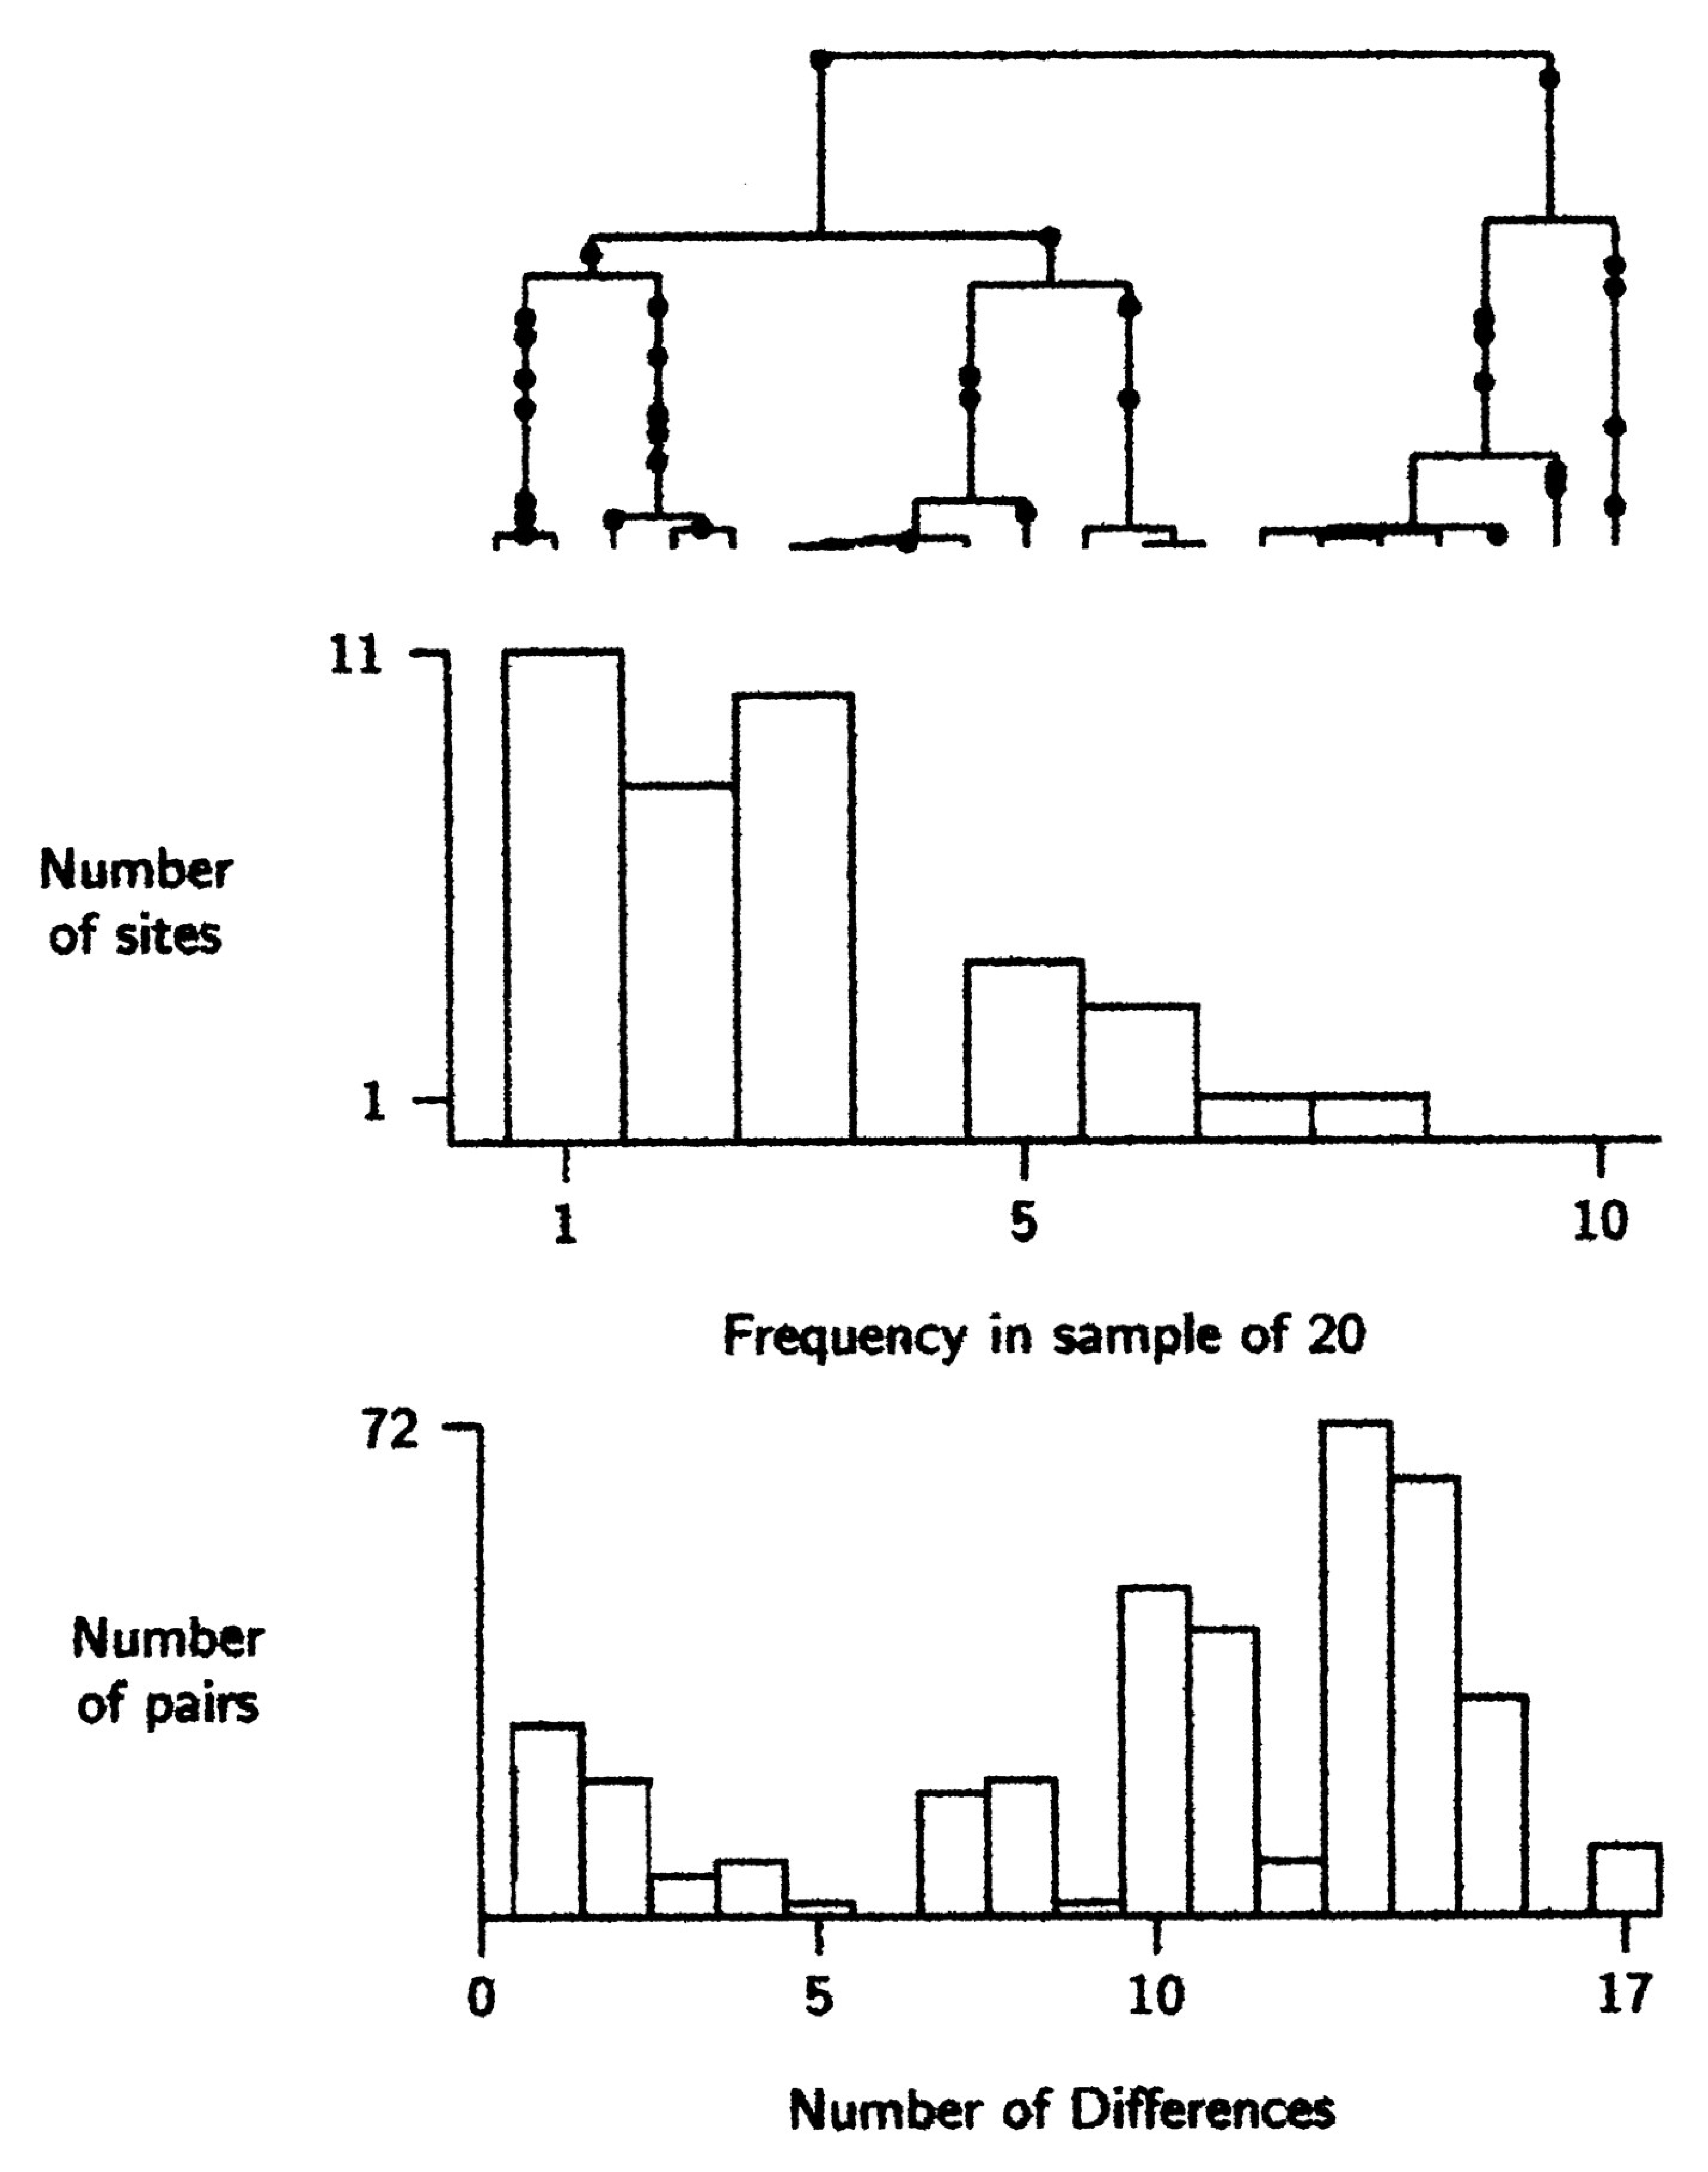
\includegraphics{mismatch-constant.eps}}
\end{center}
\caption{A gene tree (top), the frequency with which different
  haplotypes are found (middle), and the mismatch distribution
  (bottom) for a sample from a population of constant size
  (from~\cite{Harpending-etal-1998}).}\label{fig:mismatch-constant} 
\end{figure}

\begin{figure}
\begin{center}
\resizebox{!}{5cm}{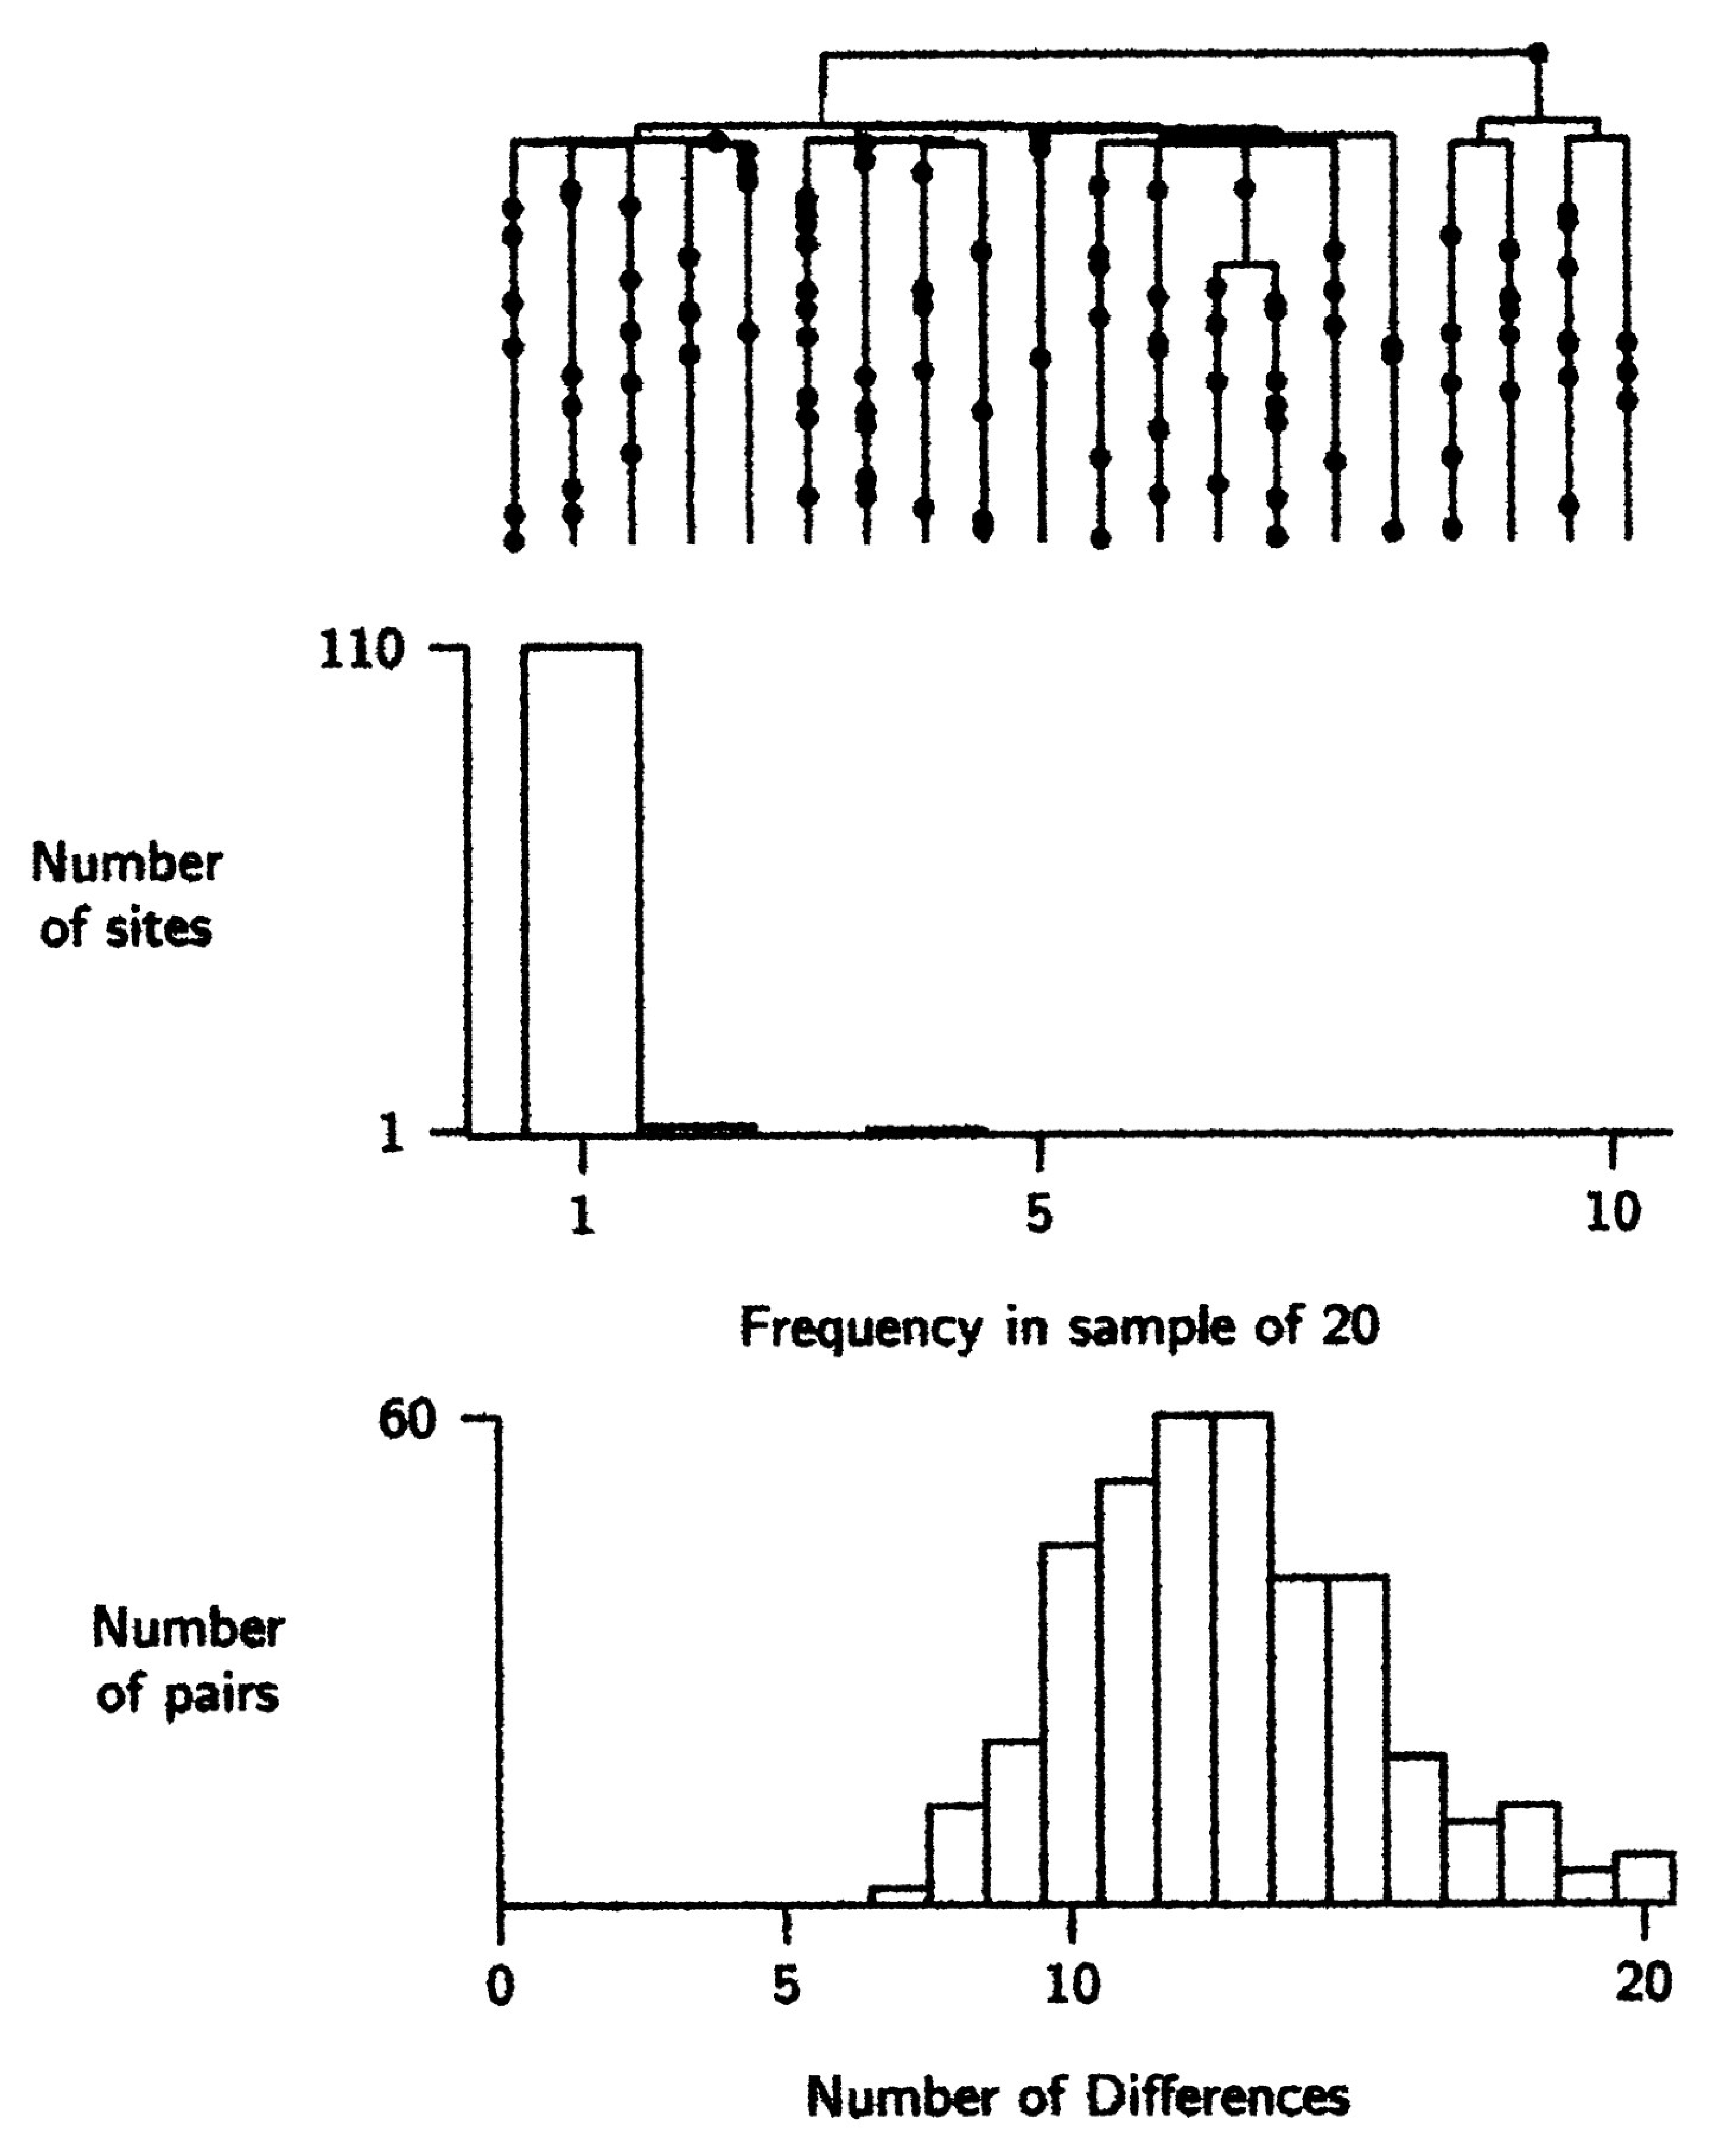
\includegraphics{mismatch-expansion.eps}}
\end{center}
\caption{A gene tree (top), the frequency with which different
  haplotypes are found (middle), and the mismatch distribution
  (bottom) for a sample from a population that has undergone a recent
  expansion
  (from~\cite{Harpending-etal-1998}).}\label{fig:mismatch-expansion}  
\end{figure}

Harpending et al.~\cite{Harpending-etal-1998} used this approach to
analyze nucleotide sequence diversity in a sample of 636 mtDNA
sequences. Their analysis focused on 411 positions in the first
hypervariable segment of human mitochondrial
DNA~(Figure~\ref{fig:mismatch-humans}). The large excess of
low-frequency variants suggests that the human population has
undergone a recent population expansion. There is, of course, the
possibility that purifying selection on the mitochondrion could
explain the pattern, so they also analyzed sequence variation on the Y
chromosome and found the same pattern. Patterns of variation at a
variety of other loci are also compatible with the hypothesis of a
recent expansion of human populations.

\begin{figure}
\begin{center}
\resizebox{!}{5cm}{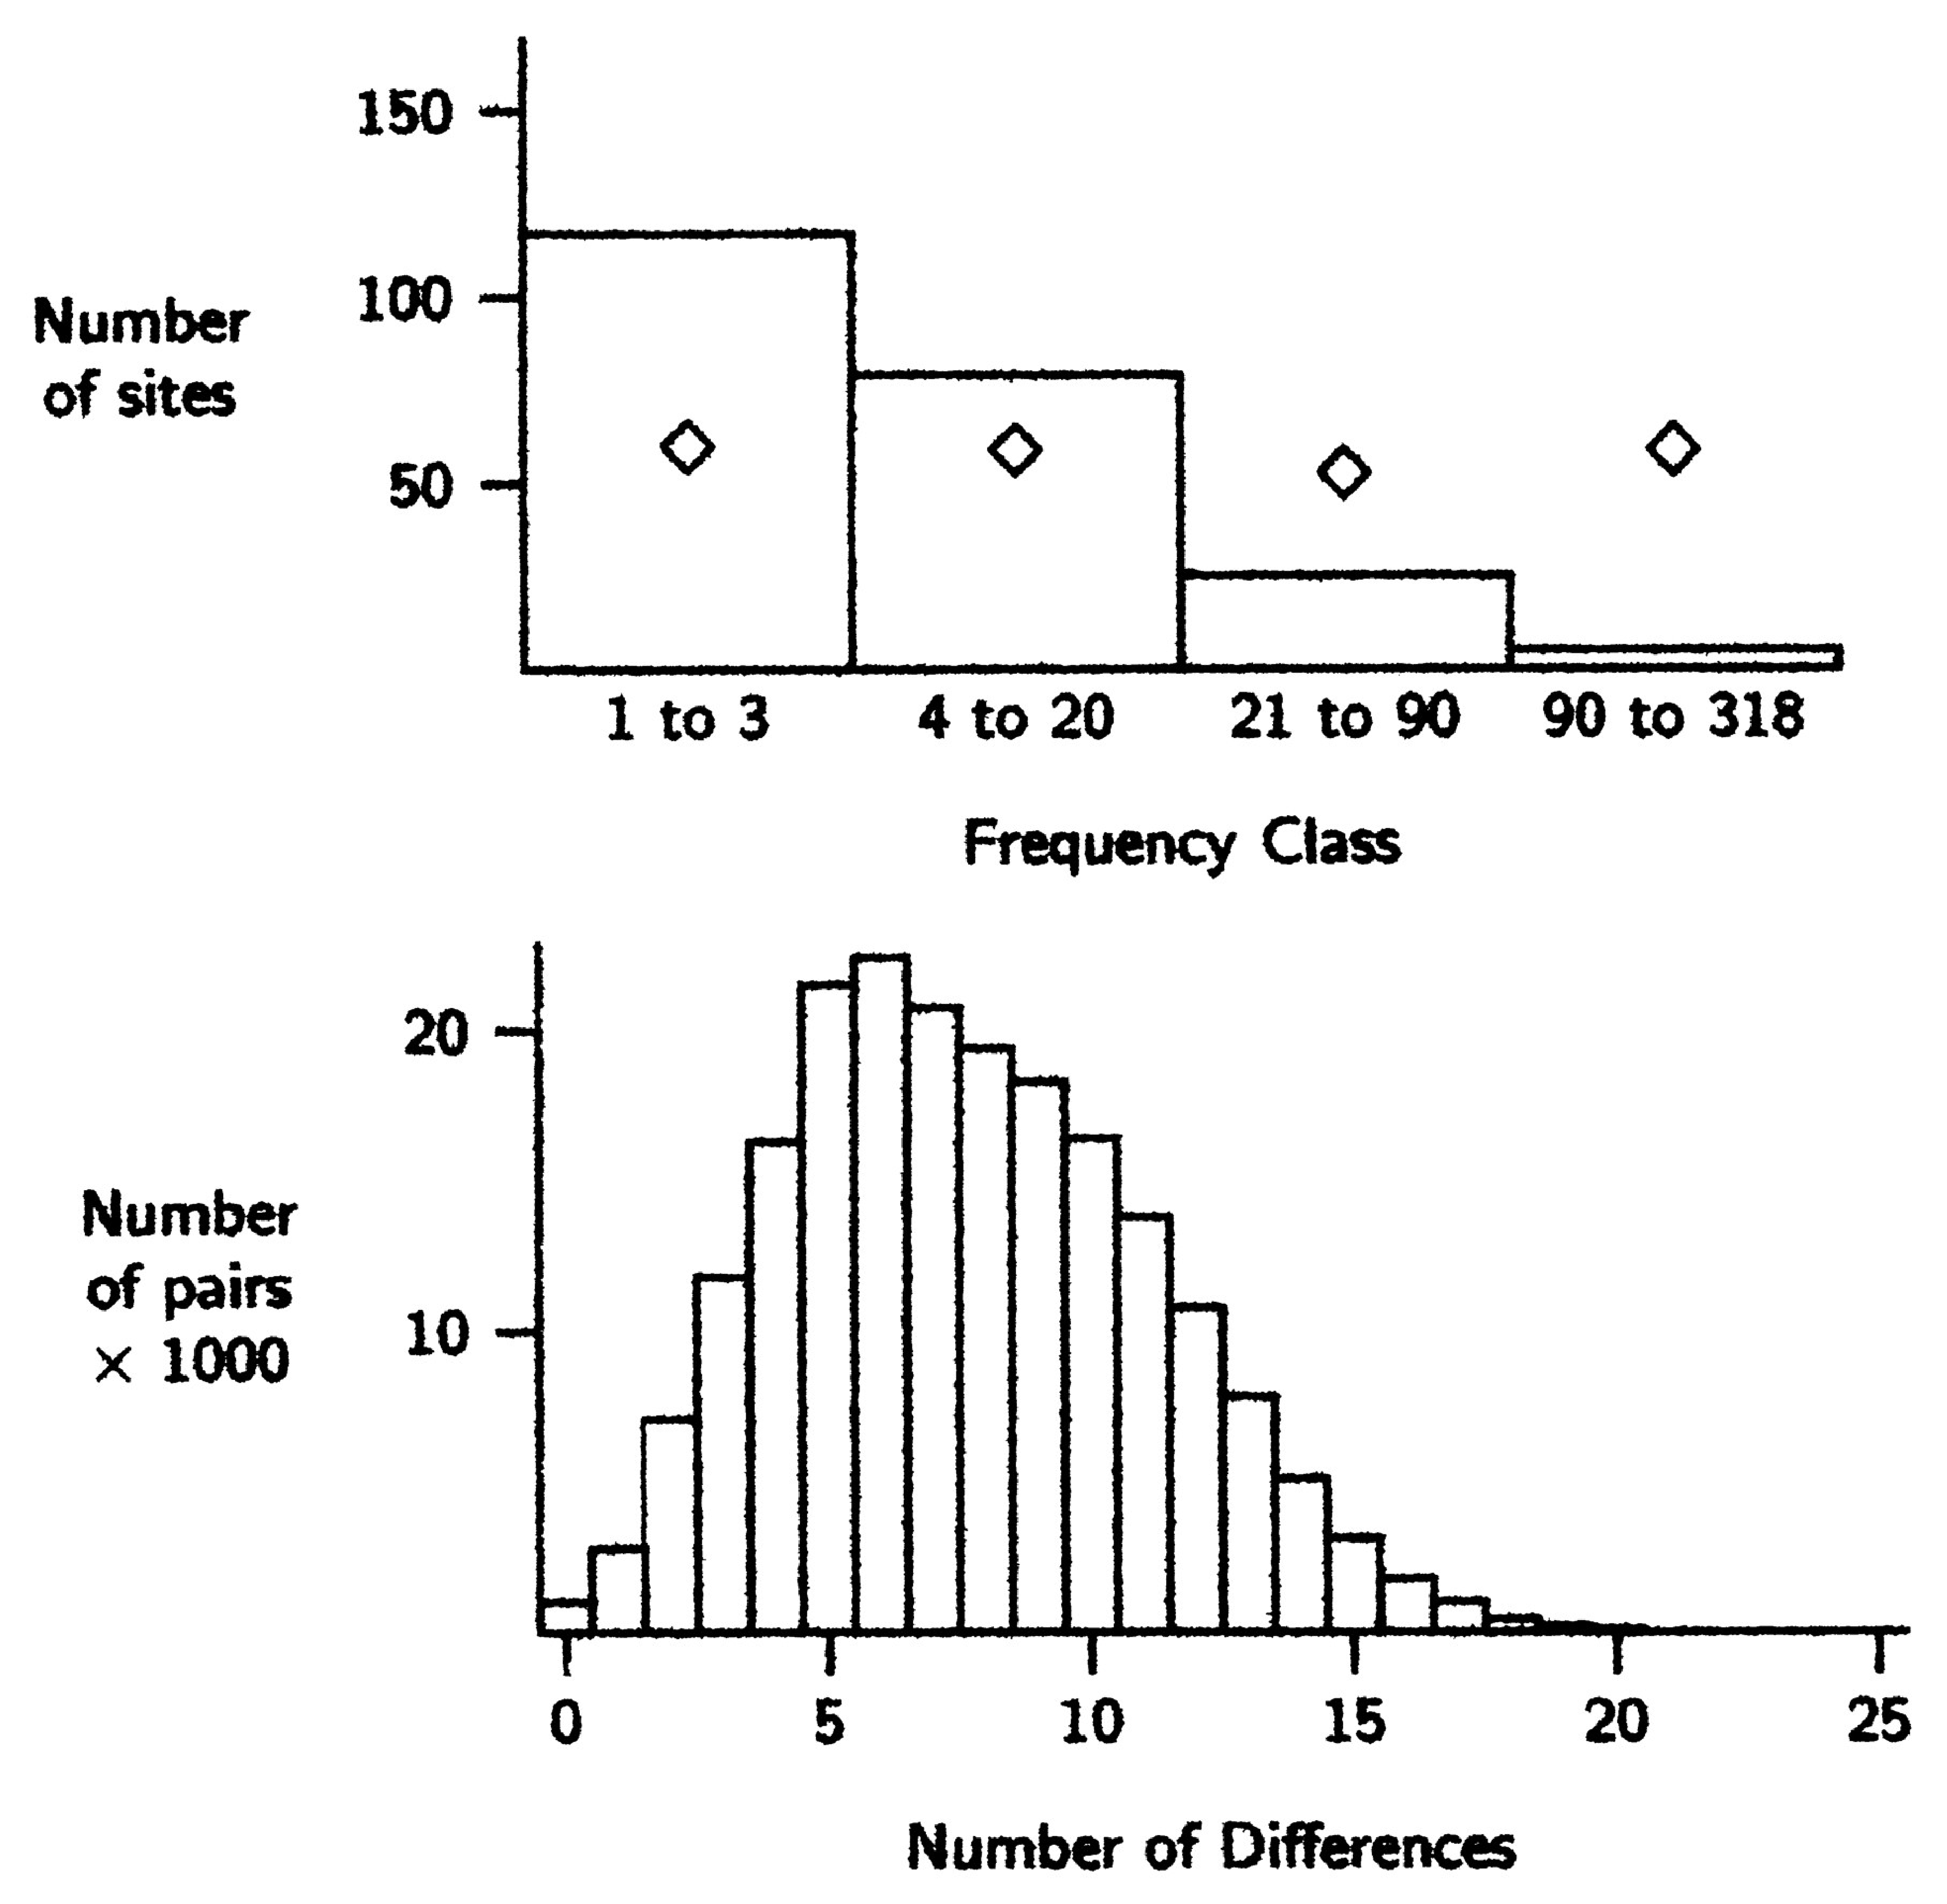
\includegraphics{mismatch-humans.eps}}
\end{center}
\caption{Mismatch distribution in a sample of 636 mtDNA sequences. The
  diamonds indicate expected values in the case of constant population 
  size (from~\cite{Harpending-etal-1998})}\label{fig:mismatch-humans} 
\end{figure}

\section*{Estimating population parameters from mismatch distributions}

Well, if we can detect recent population expansion (or contraction) in
the characteristics of the mismatch distribution, maybe we can
estimate some characteristics of the expansion. Suppose, for example,
we consider a really simple example~(Figure~\ref{fig:mismatch-model})
where the population had some constant effective size, $N_0$, and
underwent an instantaneous expansion to a new effective size, $N_1$,
some unknown time $t$ ago. We'll also assume that the mutation rate is
$\mu$,\footnote{Since we're dealing with a neutral locus, the
  substitution rate is equal to the mutation rate. This is also the
  mutation rate for the entire stretch of DNA we're looking at. In
  other words, if the per nucleotide mutation rate is $10^{-9}$ and
  our DNA sequence is a thousand nucleotides long $\mu = 10^{-9}\times
  10^3 = 10^{-6}$.} and we'll assume that we're dealing with a haploid
population, e.g., human mitochondrial DNA.

\begin{figure}
\begin{center}
\resizebox{!}{5cm}{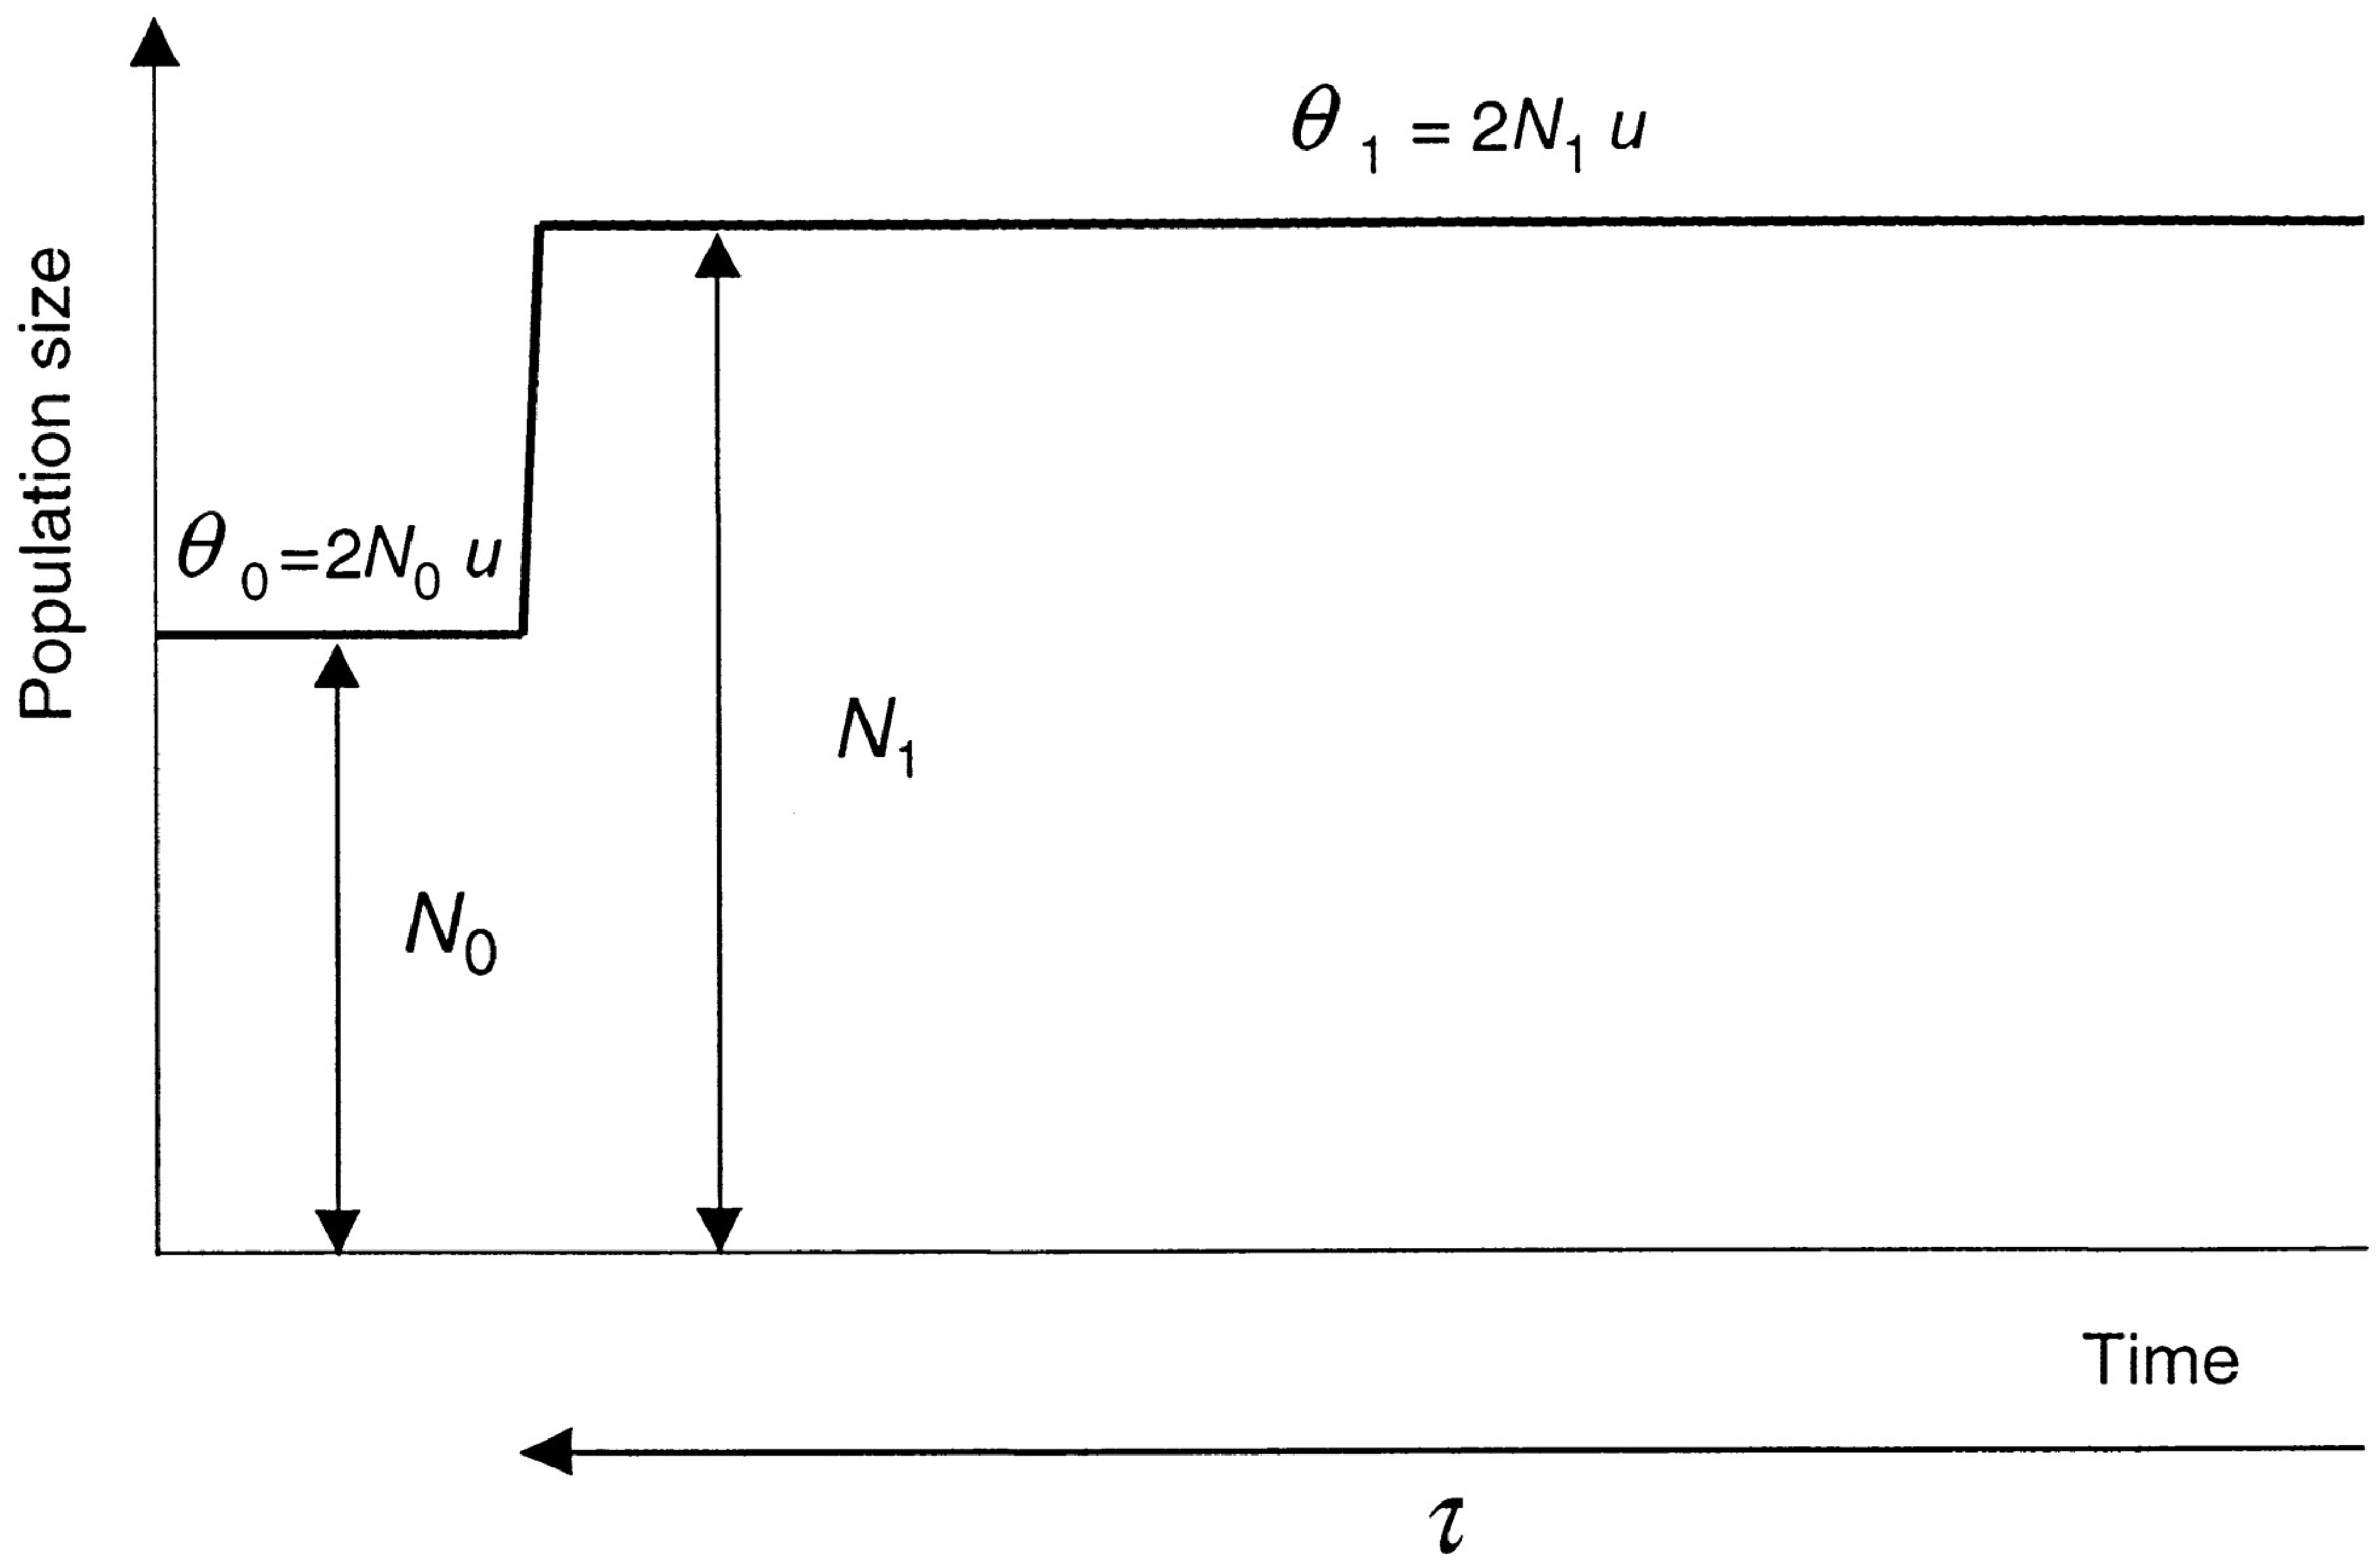
\includegraphics{mismatch-model.eps}}
\end{center}
\caption{The simple demographic scenario underlying estimation of
  population expansion parameters from the mismatch distribution
  (from~\cite{Schneider-Excoffier-1999}).}\label{fig:mismatch-model}
\end{figure}

You can probably already guess that the properties of the mismatch
distribution under this simple model depends only on the products
$N_0\mu$ and $N_1\mu$, so we'll define new parameters
$\theta_0=2N_0\mu$ and $\theta_1=2N_1\mu$ to save ourselves a little
bit of time. Similarly, we'll let $\tau = 2\mu t$. Given these
assumptions, it's possible to calculate the mismatch
distribution.\footnote{You may be astonished to learn that I'm not
  going to give you a formula for the distribution. If you're
  interested, you can find it in~\cite{Schneider-Excoffier-1999}.}
Fortunately, you don't have to calculate it yourself. {\tt Arlequin}
will take care of that for you.\footnote{And give you bootstrapped
  confidence intervals to boot!} Unfortunately, Schneider and
Excoffier~\cite{Schneider-Excoffier-1999} show that of the three
parameters we could estimate using this model, only $\tau$ is
estimated with a reasonable degree of reliability.

DNA sequence data from hypervariable region 1 (mtDNA) in a sample from
Senegalese Mandenka is distributed with {\tt Arlequin}. If we estimate
the parameters of demographic expansion, we get the results in
Table~\ref{table:mismatch-example}. The sequence in question is 406
nucleotides long. If we assume that mutations occur at a rate of
$2\times 10^{-6}$ per nucleotide per generation, then $\mu \approx
8\times 10^{-4}$, so $t \approx 3875$ generations. In other words,
according to these data the expansion took place roughly 75,000 years
ago.\footnote{If we assume that I got the mutation rate roughly
  right.}

\begin{table}
\begin{center}
\begin{tabular}{c|rr}
\hline\hline
Parameter & Mean & (99\% CI) \\
\hline
$\theta_0$ &  1.4 & (1.4, 15.4) \\
$\theta_1$ & 23.0 & (0.0, 9.2) \\
$\tau$     &  6.2 & (10.8, 99999) \\
\hline
\end{tabular}
\end{center}
\caption{Parameters of demographic expansion based on mtDNA sequence
  data distributed with {\tt Arlequin}.}\label{table:mismatch-example}
\end{table}

{\tt Arlequin} also reports two statistics that we can use to assess
whether our model is working well: the sum of squared deviations (Ssd)
and Harpending's raggedness index\footnote{A test of Tajima's $D$ will
  tell us whether we have evidence that there might have been an
  expansion. In this case, $\hat D = -1.14$ and $P=0.10$, so we have
  only weak evidence of any departure from a drift-mutation
  equilibrium.} 
\[
r = \sum_{i=1}^{d+1}(x_i - x_{i-1})^2 \quad ,
\]
where $x_i$ is the frequency of haplotypes that differ at $i$
positions and $d$ is the maximum number of observed differences. In
these data
\begin{eqnarray*}
\mbox{P}(\mbox{Expected Ssd} \ge \mbox{Observed Ssd}) &=& 0.83 \\
\mbox{P}(\mbox{Expected } r \ge \mbox{Observed } r) &=& 0.96 \quad .
\end{eqnarray*}
The large value of Harpending's $r$, in particular, suggests that the
model doesn't provide a particularly good fit to these
data.\footnote{Which is consistent with our analysis of Tajima's $D$
  that there isn't much evidence for departure from a drift-mutation
  equilibrium.} 

\bibliography{popgen}
\bibliographystyle{plain}

\ccLicense

\end{document}